\documentclass{article}
\usepackage[utf8]{inputenc}
\usepackage[brazil]{babel}
\usepackage{amsmath}
\usepackage{amssymb}
\usepackage{amsfonts}
\usepackage{graphicx}
\usepackage{float}
\usepackage[shortlabels]{enumitem}
\usepackage{fancyhdr} 
\usepackage{lastpage} 
\usepackage{amsthm}
\usepackage{multicol}
\usepackage{booktabs}
\usepackage{pgfplots}
\pgfplotsset{compat=1.18}
\usepackage{tikz}
\usepackage{wrapfig}
\usepackage{subcaption}
\usepackage[colorlinks=true, linkcolor=black, urlcolor=blue]{hyperref}

\pagestyle{fancy}
\fancyhf{} 

\lhead{
\includegraphics[height=0.29cm]{img/emap.png}} 
\rhead{\textbf{Fundação Getúlio Vargas}}

\lfoot{História da Matemática}
\rfoot{Página \thepage\ de \pageref{LastPage}} 

\renewcommand{\headrulewidth}{0.4pt}
\renewcommand{\footrulewidth}{0.4pt}

\begin{document}
\begin{titlepage}
    \centering 


    
\includegraphics[width=0.2\textwidth]{img/fgv.png} 
    
    \vspace{0.3cm} 

    {\Large FUNDAÇÃO GETULIO VARGAS \\}
    {\normalsize ESCOLA DE MATEMÁTICA APLICADA \\}
    {\normalsize História da Matemática}

    \vfill 

    {\bfseries\Large Logaritmo e suas Aplicações }

    \vfill 

    \begin{tabular}{c}
        RODRIGO SEVERO ARAÚJO\\
        VICTOR GABRIEL HARUO IWAMOTO \\
    \end{tabular}

    \vspace{2.cm} 

    {Rio de Janeiro -- RJ \\} 
    {Outubro 2025}

\end{titlepage}
\section{Tábua de Logaritmo}


A capacidade computacional hodierna banalizou operações que antes representavam desafios consideráveis de tempo e precisão, como o produto $4538 \cdot 675$. Entretanto, até a disseminação das calculadoras eletrônicas na década de 1970, tal cálculo exigia métodos analógicos e tabulares. Na época, a solução era advinda de métodos que utilizavam tábuas de logaritmos e réguas de cálculo.

\begin{figure}[H]
    \centering
    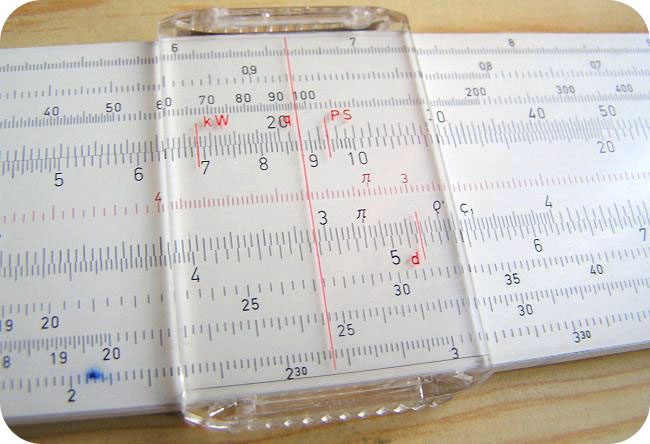
\includegraphics[height=6cm]{img/regua.png}
    \caption{Régua de Cálculo}
\end{figure}

\subsection{Exemplo}

Para elucidar o método, demonstraremos como as tábuas eram utilizadas para computar o produto $4538\cdot 675$. O método se fundamenta a partir da seguinte propriedade de logaritmo:

\begin{align*}
    P = a \cdot b \quad & \implies \quad \log(P) = \log(a \cdot b) \\
                       & \implies \quad \log(P) = \log(a) + \log(b) \\
                       & \implies \quad P = \log^{-1}\left( \log(a) + \log(b) \right)
\end{align*}

\textbf{Tabelas do Exemplo:}
\begin{figure}[H]
    \centering
    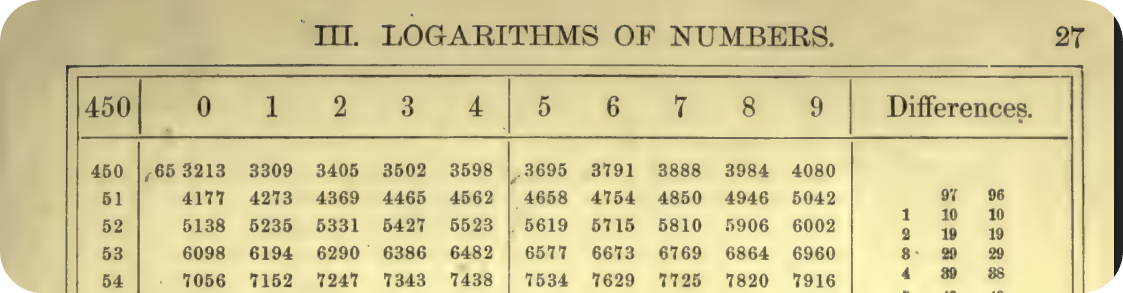
\includegraphics[height=3cm]{img/4538.png}
    \caption{Tabela do Número 4538}
\end{figure}

\begin{figure}[H]
    \centering
    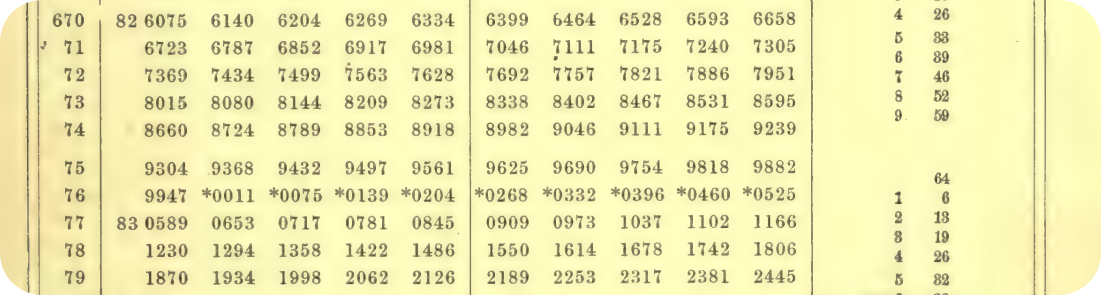
\includegraphics[height=3cm]{img/675.png}
    \caption{Tabela do Número 675}
\end{figure}

\begin{figure}[H]
    \centering
    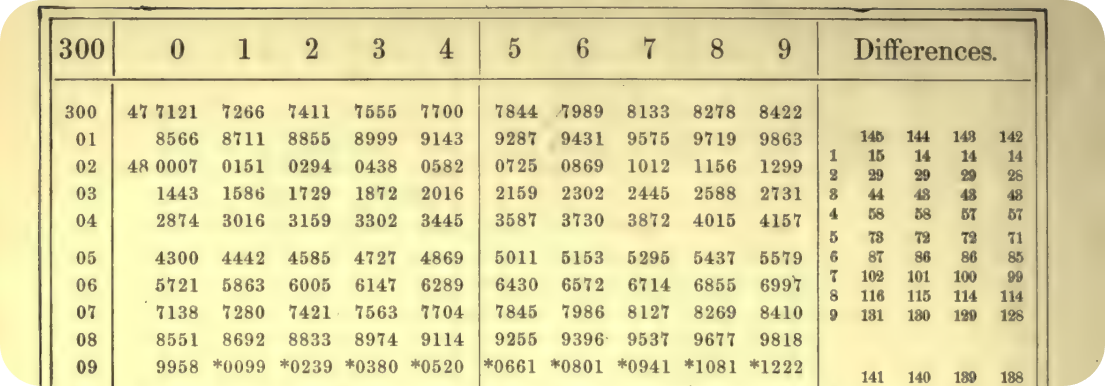
\includegraphics[height=4cm]{img/res.png}
    \caption{Tabela do Número Resultado}
\end{figure}

Para fins de organização separemos o método em etapas:

\begin{itemize}
    \item Passo 1: Computar o logaritmo dos números 4538 e 675
    \item Passo 2: Somar o resultado encontrado
    \item Passo 3: Encontrar o antilogaritmo do resultado
    \item Passo 4: Aplicar métodos de interpolação para melhorar o resultado.
\end{itemize}

\subsubsection{Passo 1}
A princípio, é necessário computar o logaritmo dos número 4538 e 675. Mostraremos o processo para o número 4538 e para o número 675 é análogo e fica como exercício para o leitor. O método pode ser particionado em encontrar a parte inteira e a parte fracionária do logaritmo desejado, denota-se característica e mantissa respectivamente.

\textbf{Parte Inteira:}
Note que:
\begin{align*}
    & 10^3 \le 4538 \le 10^4 \iff \\
    & \log(10^3) \le \log(4538) \le \log(10^4) \iff \\
    & 3 \le \log(4538) \le 4
\end{align*}

Daí, a parte inteira do $\log(4538)$ é 3.

\textbf{Mantissa:}
Para a mantissa é necessário consultar a tábua presente na Figura 2. Em suma, basta encontrar os primeiros digitos do valor desejado (450) e veja que os algarismos da parte superior da tábua é referente ao último digito, isto é, no exemplo devemos consultar a coluna do 8. Além disso, nesse exemplar é omitido as duas primeiras casas decimais da mantissa, nessa tábua tais valores estão precedentes à coluna do algarismo 0, isto é, no exemplo, já juntando os digitos, a mantissa é 656864.

Para descobrir a mantissa do valor 675 faça o uso da tábua presente na Figura 3.

Daí, $\log(4538) \approx 3,656864$ e $\log(675) \approx 2,829304$.

\subsubsection{Passo 2}

Somando os valores encontrados no passo anterior, temos que:
\begin{align*}
    \log(4538 \cdot 675) &= \log(4538) + \log(675) \\
                        &\approx 3{,}656864 + 2{,}829304 \\
                        &= 6{,}486168
\end{align*}

\subsubsection{Passo 3}
De maneira análoga, encontrar o antilogaritmo segue o mesmo método.

\textbf{Parte Inteira:}

\begin{align*}
    & 6 \le 6{,}486168 \le 7 \iff \\
    & \log^{-1}(6) \le \log^{-1}(6{,}486168) \le \log^{-1}(7) \iff \\
    & 10^6 \le 4538 \cdot 675 \le 10^7
\end{align*}

Daí, a parte inteira indica que o resultado está na casa dos milhões ($10^6$).

\textbf{Mantissa:}
Por meio da tábua na Figura 4, procuremos os dois primeiros digitos da mantissa (48), como logaritmo é uma função crescente, basta procurar ordenadamente. Daí, nos valores que englobam o 48 procuremos pelo piso de 6168. Veja que, como não há o número exato, o número se encontra no intervalo $[6147, 6289]$. Assim, ao tomar 6147 encontramos que o valor aproximado do antilogaritmo desejado é 3063.

Juntando a informação obtida a partir da parte inteira e da mantissa chegamos que $4538 \cdot 675 = 3.063.000$. Por meio de ferramentas de computacionais hodierna descobrimos que o produto é na verdade 3063150; assim, o erro percentual relativo é 0,0049\% .

\subsubsection{Passo 4}

Não satisfeito com a aproximação anterior, ainda por meio da tábua há a possibilidade de melhorar o resultado.

No passo precedente, vimos que $6168 \in I=[6147, 6289]$, assim, $|I| = 142$ e a diferença do valor desejado para o extremo esquerdo de I é $6168-6147 = 21$. Dessa maneira, analisando a parte de diferença da tabela na coluna $142$, vemos que $21 \in [14,28]$, melhor dizendo, o quinto dígito é 1, já que devemos sempre pegar o mínimo do menor intervalo possível. Assim, o resultado do produto se torna 3.063.100.

Para descobrirmos o sexto dígitos é necessário realizar um truque, note que no processo anterior na tabela das diferenças não encontramos exatamente o número 21, então podemos subtrair o valor desejado pelo extremo esquerdo do intervalo, $21-14 = 7$ (denotaremos de resto). Além disso, computamos o tamanho do intervalo, isto é, $28-14 = 14$ (denotaremos de intervalo). Daí, utilizando a seguinte fórmula:

\begin{align*}
    \dfrac{Resto}{Intervalo} = 7/14 = 0.5
\end{align*}

O resultado nos dá o sexto digito, assim, o resultado do produto se torna 3.063.150

\subsubsection{Conclusão}
Veja que após realizar o processo de interpolação duas vezes consecutivas reduzimos o erro percentual relativo para zero, isto é, encontramos o resultado exato. Demonstrando que apesar de trabalhoso o método realmente é funcional.
\section{Motivação e Contexto Histórico}
\newpage
\section{Outras Vertentes}

\subsection{Henry Briggs}
\begin{wrapfigure}{l}{0.3\textwidth}
    \setlength{\intextsep}{0pt}
    \vspace{-1.5em} 
    \centering
    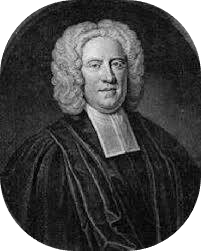
\includegraphics[width=\linewidth]{img/briggs.png} 
\end{wrapfigure}

Em 1616, impulsionado pela repercussão dos logaritmos, o matemático inglês Henry Briggs (1561 - 1630), professor de geometria no Gresham College, em Londres, ficou fascinado com a criação de Napier. Briggs visitou Napier em Edimburgo e sugeriu uma alteração na base do logaritmo. Com o intuito de tornar os cálculos mais intuitivos, ele propôs que o logaritmo fosse calculado na base decimal.

Napier concordou com a ideia; entretanto, faleceu logo em seguida, em 1617. Dessa forma, o encargo de adaptar as tabelas de logaritmos para a base decimal ficou a cargo de Briggs.

Em 1617, Briggs publicou os logaritmos dos primeiros 1.000 números. Já em 1624, lançou o livro \textit{Arithmetica Logarithmica}, uma obra contendo os logaritmos dos primeiros 30.000 números naturais, com 14 casas de precisão.

\begin{figure}[H]
    \centering
    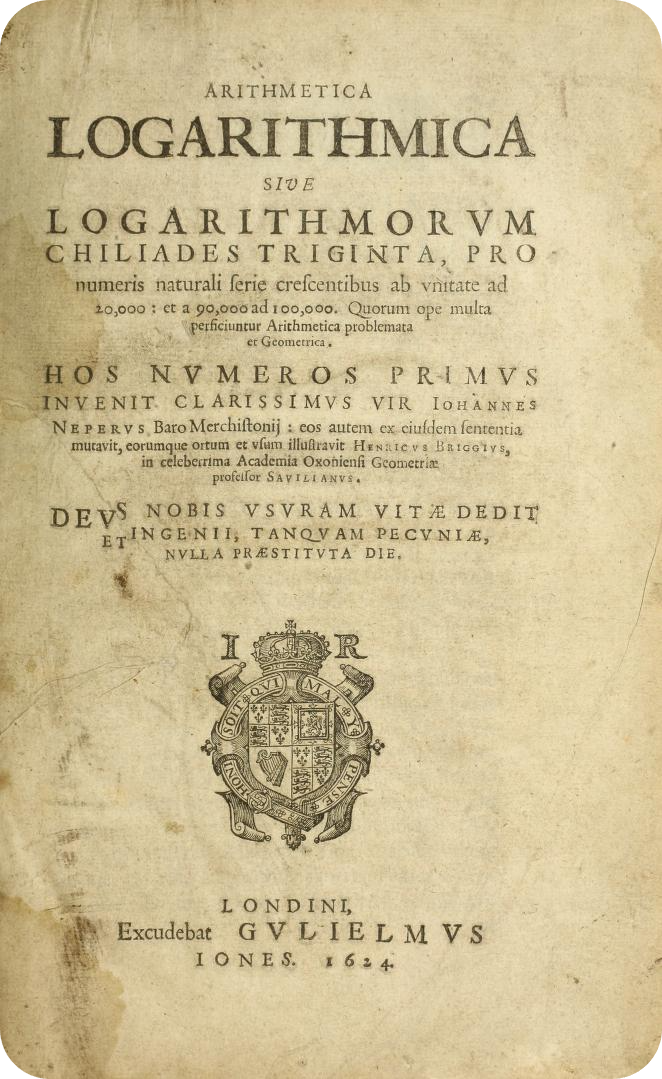
\includegraphics[height=9cm]{img/capa.png}
    \caption{Capa do Arithmetica Logarithmica}
\end{figure}

\begin{figure}[H]
    \centering
    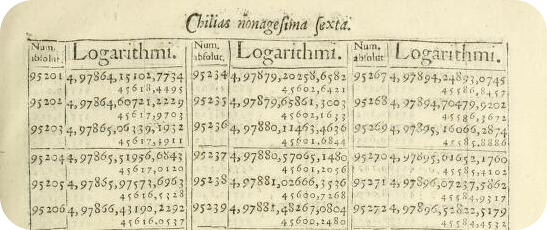
\includegraphics[height=4.5cm]{img/tabela1.png}
    \caption{Tabela desenvolvida por Briggs}
\end{figure}

\subsection{Jost Burgi}

\begin{wrapfigure}{l}{0.3\textwidth}
    \setlength{\intextsep}{0pt}
    \vspace{-1.5em} 
    \centering
    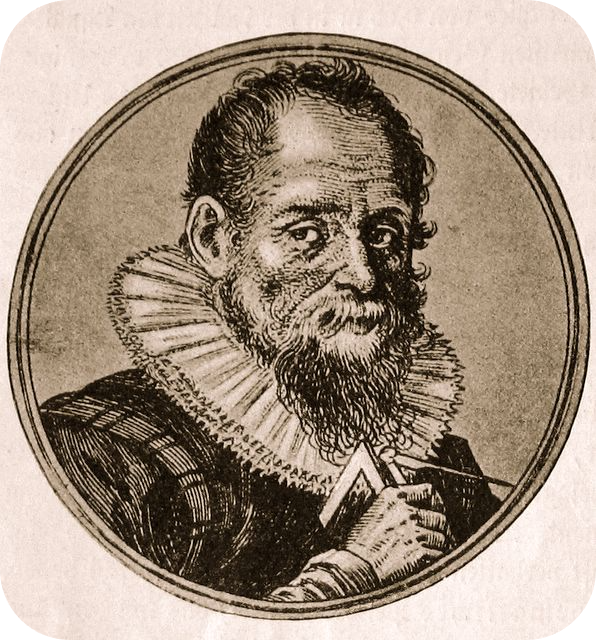
\includegraphics[width=\linewidth]{img/burgi.png} 
\end{wrapfigure} 

Por volta de 1600, o relojoeiro e matemático suíço Jost Bürgi (1552-1632) construiu uma tabela de progressões (um conceito análogo aos antilogaritmos) que precedeu os trabalhos de Napier, utilizando um método distinto. 

Ao desenvolver sua tabela, Burgi percebeu que utilizar bases simples, como por exemplo 2, fazia com que as potências crescessem muito rapidamente e, portanto, tornando impraticável seu uso para interpolação de valores. Como método de contornar tal problemática, Burgi adotou uma razão muito próxima de 1, em específico $1.0001$ como base para sua progressão geométrica.

Um dos aspectos mais distintos do sistema de Bürgi foi o uso de cores para enfatizar a relação dual entre a progressão aritmética (os logaritmos) e a progressão geométrica (os antilogaritmos).

Ao contrário de Napier, que desenvolveu uma terminologia técnica, Bürgi criou uma distinção visual imediata ao utilizar tinta preta e vermelha, tanto no texto explicativo quanto nas próprias tabelas:

\begin{itemize}
    \item \textbf{Números Vermelhos (Logaritmos):} Impressos em vermelho, representavam os argumentos da tabulação. Estes números seguiam uma progressão aritmética.
    
    \item \textbf{Números Pretos (Antilogaritmos):} Impressos em preto, representavam as entradas tabulares, ou os "números ordinários". Estes números seguiam a progressão geométrica de base $1.0001$.
\end{itemize}

\begin{figure}[H]
    \centering
    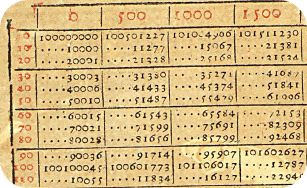
\includegraphics[height=5.5cm]{img/tabelaburgi.png}
    \caption{Tabela desenvolvida por Burgi}
\end{figure}

Apesar de a tabela de Bürgi ter, na prática, o mesmo propósito da de Napier — transformar multiplicações complexas em adições simples — e de ter sido criada anteriormente, ela não conseguiu estabelecer uma base teórica suficientemente clara para definir o conceito abstrato de função logarítmica.

Por essa razão histórica, e pela fundamentação conceitual mais robusta de seu trabalho publicado em 1614, John Napier é predominantemente reconhecido como o inventor dos logaritmos.
\section{Definição Geométrica}

Napier, em seus estudos, também desenvolveu uma definição geométrica para o logaritmo. 
Considere um segmento de reta $AB$ e uma semirreta $DE$, de origem $D$, conforme a figura \ref{fig:defgeolog}. 
Suponhamos que os pontos $C$ e $F$ se ponham em movimento simultaneamente a partir de $A$ e $D$, respectivamente, 
ao longo dessas linhas, com a mesma velocidade inicial. 
Admitamos que $C$ se mova com uma velocidade numericamente sempre igual à distância $CB$, 
e que $F$ se mova com velocidade uniforme. 

\begin{figure}[h!]
    \centering
    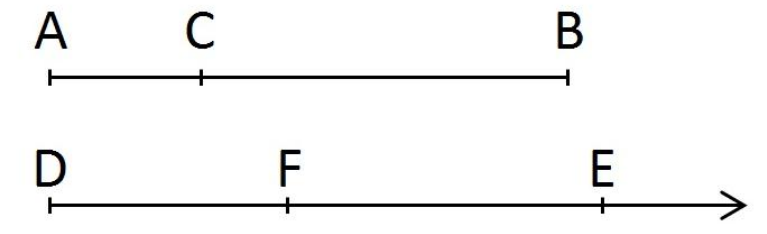
\includegraphics[width=0.4\linewidth]{img/defgeo.png}
    \caption{Definição Geométrica de logaritmo}
    \label{fig:defgeolog}
\end{figure}

Napier definiu então $DF$ como logaritmo de $CB$. 
Isto é, pondo $DF = x$ e $CB = y$, temos:

\[
x = \text{Naplog}\, y
\]

Para demonstrar esse fato, utilizaremos ferramentas do cálculo diferencial e integral que temos atualmente. Tomando $AB = 10^7$, $x=DF$, $y = CB$, sabemos que a velocidade de $C$ é a derivada de seu deslocamento, ou seja, temos que:

\[
\dfrac{d}{dt}(10^7 - y) = y \iff -\dfrac{dy}{dt} = y
\]

Resolvendo essa equação diferencial, temos que $y(t) = Ce^{-t}$, como $y(0) = C = 10^7$, segue que:

\[
y(t) = 10^7 e^{-t}
\]

Além disso, como $x(t)$ tem velocidade constante, $x(t)= 10^7 t$. Daí, obtemos as seguintes funções de deslocamento:

\[
y(t) = 10^7 e^{-t} \qquad \text{e} \qquad x(t)= 10^7 t
\]

Portanto, obtemos que:

\[
x = 10^7 t = 10^7 \cdot \text{ln}\left(\frac{10^7}{y}\right)
\]

Observe que as definições não coincidem exatamente, mas como Napier tomou $10^7$, isto é, um número muito grande. As definições são aproximadamente equivalentes. De fato, após algumas manipulações algébricas e utilizando que $\text{ln}\left(1-\frac{1}{10^7}\right) \approx -\frac{1}{10^7}$, conseguimos obter que:

\[
y = 10^7 (1-10^{-7})^{x} \implies x \approx 10^7 \text{ln}\left(\frac{10^7}{y}\right)
\]

Para visualizar essa definição geométrica, fizemos uma construção geométrica no \textit{geogebra}. Para melhor visualização utilizamos $AB = 10$. O ponto $P$ desliza sobre o plano $\mathbb{R}^2$ de modo que $P = (CB(t), DF(t))$, assim, conseguimos visualizar que isso constrói um gráfico de uma função logarítimica. Segue o link: 
\href{https://www.geogebra.org/classic/hjcec98z}{Clique Aqui}.

\begin{figure}[H]
    \centering
    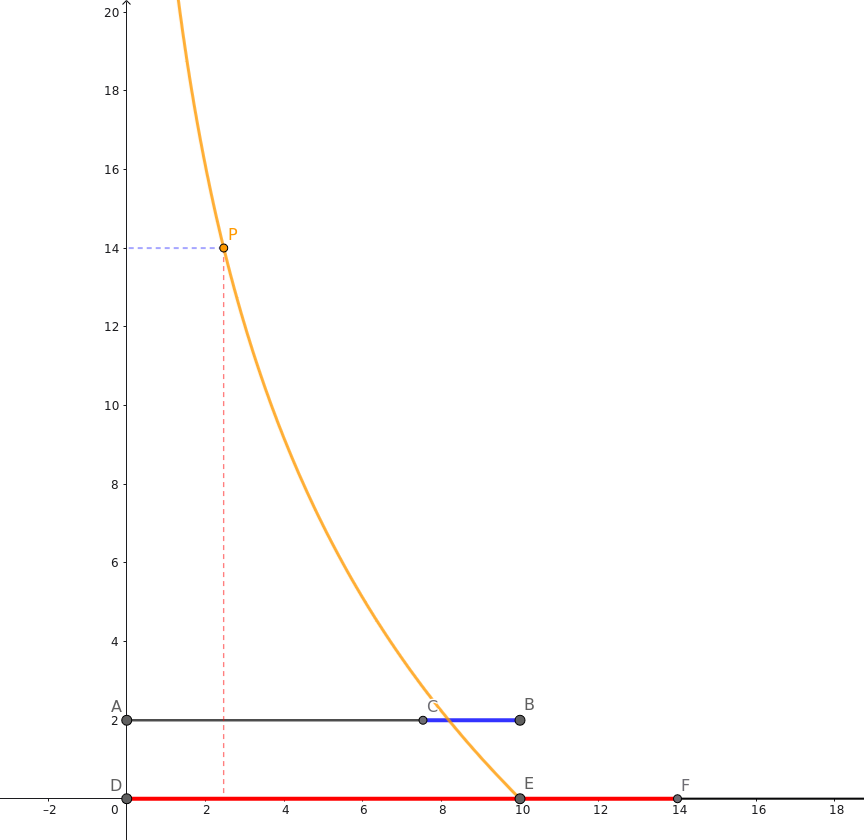
\includegraphics[width=0.9\linewidth]{img/defgeogebra.png}
    \caption{Ilustração da definição geométrica de logaritmo}
\end{figure}


\section{Definição Atual}

Apesar da enorme importância dos logaritmos para cálculos numéricos, não é dessa maneira que somos introduzidos aos logaritmos na escola. Na verdade, a definição de logaritmo que aprendemos é intimamente ligada a uma exponencial. A definição é a que segue

\textbf{Definição.} Sendo $a$ e $b$ números reais e positivos, com $a \neq 1$, chama-se \textit{logaritmo} de $b$ na base $a$ o expoente que se deve dar à base $a$ de modo que a potência obtida seja igual a $b$.
Em símbolos: se $a, b \in \mathbb{R}$, $0 < a \neq 1$ e $b > 0$, então:

\[
\log_{a} b = x \iff a^x = b
\]

A partir desta definição, é tranquilo chegarmos em algumas propriedades interessantes, não iremos prová-las pois não está no escopo do texto, porém, é um excelente exercício para o leitor.

\vspace{8pt}
\noindent\textbf{\underline{Propriedades dos logaritmos:}}

\begin{multicols}{2}
\begin{enumerate}
    \item ${a^{\log_a x} = x}$  
    \item ${\log_a a^k = k}$  
    \item ${\log_a 1 = 0}$ 
    \item ${\log_a a = 1}$ 
    \item ${\log_a x^k = k \log_a x}$ 
    \item ${\log_a(x\cdot y) = \log_a x + \log_a y}$ 
    \item ${\log_a\!\left(\dfrac{x}{y}\right) = \log_a x - \log_a y}$
    \item ${\log_a x = \dfrac{\log_b x}{\log_b a}}$ 
\end{enumerate}
\end{multicols}



\section{O Logaritmo Hiperbólico}

Décadas depois da invenção de Napier, em 1647 os logaritmos apareceram em um campo não esperado, na \textbf{área de uma hipérbole}.

Vamos focar o estudo na hipérbole quadrada, isto é, a hipérbole $xy = 1$, ou ainda, $y = \frac{1}{x}$. Queremos estudar a área abaixo do gráfico de $1$ a algum ponto $a$ no eixo $x$. Utilizando linguagem atual do cálculo, queremos estudar:
\[
A(a) = \int_1^a \frac{1}{x} dx
\]

A figura \ref{fig:abaixohiperbole} mostra a área que estamos interessados 

\begin{figure}[H]
    \centering
    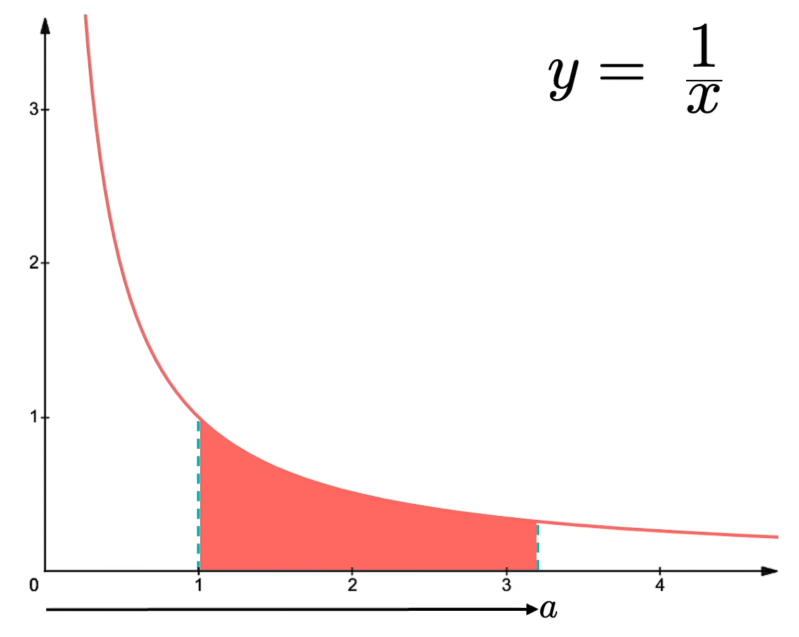
\includegraphics[width=0.5\linewidth]{img/areaabaixohip.png}
    \caption{Área abaixo da Hipérbole de $1$ a $a$}
    \label{fig:abaixohiperbole}
\end{figure}

\begin{wrapfigure}{l}{0.3\textwidth}
    \setlength{\intextsep}{0pt}
    \vspace{-1.5em} 
    \centering
    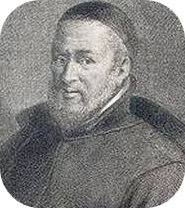
\includegraphics[width=\linewidth]{img/SaintVincent.png}
    \caption*{Saint Vincent}
\end{wrapfigure}

Calcular essa área se mostrou uma atividade difícil, pois muitos matemáticos tentaram calcular esta área e falharam, entre eles estão Arquimedes, René Descartes e Fermat. Fermat abriu caminho para que o matemático Grégoire de Saint-Vincent (1584 - 1667) finalmente descobrisse a àrea abaixo da hipérbole.

Para calcular essa área, Saint-Vincent a dividiu em retângulos de uma maneira particular, ilustrada na figura \ref{fig:hiperbole}.
O 1° retângulo começa no ponto $a$, o 2° retângulo começa no ponto $ar$, o 3° em $ar^2$ e assim por diante, até chegar em $1$, além disso, note que $r < 1$. A ideia era clara, somar a área de todos os retângulos. Entretanto, não é difícil ver que há um erro com a área real, porém, se $r$ estiver suficientemente próximo de $1$, este erro fica imperceptível.

\begin{figure}[H]
    \centering
    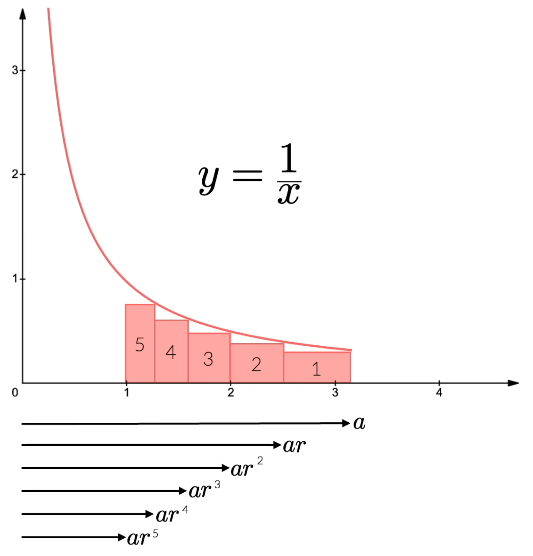
\includegraphics[width=0.5\linewidth]{img/hiperbole.png}
    \caption{Área da Hipérbole via progressão geométrica}
    \label{fig:hiperbole}
\end{figure}

Iremos calcular as áreas destes retângulo para ver se encontramos algo interessante, os resultados estão na tabela \ref{tab:areasvincent}

\begin{table}[h!]
\centering
\begin{tabular}{c c c c}
\toprule
\textbf{Retângulo} & \textbf{Altura} & \textbf{Comprimento} & \textbf{Área} \\
\midrule
1 & $\dfrac{1}{a}$ & $a(1-r)$ & $(1-r)$ \\
\addlinespace
2 & $\dfrac{1}{ar}$ & $ar(1-r)$ & $(1-r)$ \\
\addlinespace
3 & $\dfrac{1}{ar^2}$ & $ar^2(1-r)$ & $(1-r)$ \\
\addlinespace
4 & $\dfrac{1}{ar^3}$ & $ar^3(1-r)$ & $(1-r)$ \\
\addlinespace
5 & $\dfrac{1}{ar^4}$ & $ar^4(1-r)$ & $(1-r)$ \\
\bottomrule
\end{tabular}
\caption{Tabela de Retângulos sob a curva $y=1/x$}
\label{tab:areasvincent}
\end{table}

Encontramos algo interessante! As áreas de cada um desses retângulos são exatamente as mesmas, todas iguais a $(1-r)$. Esse resultado deu Saint-Vincent a seguinte ideia: ele percebeu que isso levava a uma interessante relação entre a distância e a área abaixo da hipérbole, ilustrada na tabela \ref{tab:distarea}.


\begin{table}[h!]
\centering
\begin{tabular}{c c}
\toprule
\textbf{Distância} & \textbf{Área} \\
\midrule
$ar^5$ & $0$ \\
\addlinespace
$ar^4$ & $(1-r)$ \\
\addlinespace
$ar^3$ & $2(1-r)$ \\
\addlinespace
$ar^2$ & $3(1-r)$ \\
\addlinespace
$ar$ & $4(1-r)$ \\
\addlinespace
$a$ & $5(1-r)$ \\
\bottomrule
\end{tabular}
\caption{Relação entre distância e área abaixo da hipérbole}
\label{tab:distarea}
\end{table}

Observe que na distância, de uma linha para outra multiplicamos sempre por $1/r$, enquanto na área somamos sempre $(1-r)$  Isso significa que a distância está seguindo uma progressão geométrica, enquanto a área está seguindo uma progressão aritmética.

Logo, os números na tabela relacionados seguem as mesmas ideias vistas por Napier anos antes. E portanto a relação entre a distância e a área é \textit{logarítmica}.

Daí, Alfonso de Sarasa, um dos estudantes de Saint Vincent, escreveu essa relação de forma explícita, a área da hipérbole até o ponto $a$, foi definida como

\[
A(a) = \log(a)
\]

Esse logaritmo foi chamado de \textbf{logaritmo hiperbólico}. Porém, Saint Vincent e de Sarasa ainda não foram capazes de encontrar uma maneira para calculá-lo. Daí entra uma nova figura: Nicholas Mercator.

\section{Série de Mercator}

Ainda no espectro da matemática, após a descoberta da íntima conexão entre a função logaritmo e área sobre a hipérbole começaram a surgir consequências da propriedade. 

A Série de Mercator é um dos principais marcos. Inicialmente, a série foi descoberta independemente por Johannes Hudde (1656) e por Isaac Newton (1665), entretanto, nenhum dos dois havia publicado o resultado. Apenas em 1668, Nicholas Mercator após descobrir de forma independente publicou o seu tratado Logarithmotechnia com a seguinte série:

\begin{equation*}
    \ln(1+x) = x - \dfrac{x^2}{2} + \dfrac{x^3}{3} - \dfrac{x^4}{4} + \ldots
\end{equation*}

que aproxima a função logaritmo para o intervalo $-1<x \le 1$.

\subsection{Demonstração}

Note que a propriedade de a área da hipérbole se relacionar ao logaritmo pode ser resumida em: 
\begin{equation}
    \ln(1+x) = \int_{0}^{x}\dfrac{1}{1+t}dt
\end{equation}


Na época de Mercator, as séries geométricas já eram difundidas, daí os matemáticos da época já conheciam a seguinte expressão:

\begin{equation} \label{eq:serie_geo}
    \frac{1}{1-x} = 1 + x+x^2+x^3 + \ldots
\end{equation}

Ao analisar a expressão dentro da integral, Mercator percebeu que a expressão (\ref{eq:serie_geo}) ao tomar $x = -t$ se torna:

\begin{equation}
    \dfrac{1}{1+t} = 1 -t+t^2-t^3 + \ldots
\end{equation}

Daí:

\begin{equation}
    \ln(1+x) = \int_{0}^{x}\dfrac{1}{1+t}dt = \int_{0}^{x} 1 -t+t^2-t^3 + \ldots dt
\end{equation}


Como a integral em (4) é polinomial, é facil calcular a primitiva:

\begin{align*}
    \int_{0}^{x} (1 -t+t^2-t^3 + \ldots) \,dt &= \left[ t - \frac{t^2}{2} + \frac{t^3}{3} - \frac{t^4}{4} + \ldots \right]_{0}^{x} \\
                                              &= x - \frac{x^2}{2} + \frac{x^3}{3} - \frac{x^4}{4} + \ldots
\end{align*}

Note que, o resultado nada mais é do que um caso específico da Série de Taylor com $f(x) = \ln(1+x)$ em $x=0$.

\begin{equation*}
    f(x) = \sum_{n=0}^{\infty} a_n (x-a)^n \qquad \text{sendo} \qquad a_n = \frac{f^{(n)}(a)}{n!}
\end{equation*}

Ao calcular as derivadas consecutivas:
\begin{align*}
    f(x) &= \ln(1+x) \\
    f'(x) &= \frac{1}{1+x} \\
    f''(x) &= -\frac{1}{(1+x)^2} \\
    f^{(3)}(x) &= \frac{2}{(1+x)^3} \\
    f^{(4)}(x) &= -\frac{6}{(1+x)^4} \\
    &\vdots
\end{align*}

Agora, avaliamos tudo em $x=0$:

\[
f(0) = 0, \quad f'(0) = 1, \quad f''(0) = -1, \quad f^{(3)}(0) = 2, \quad f^{(4)}(0) = -6, \ldots
\]

Por fim, substituindo:
\begin{align*}
    \ln(1+x) &= f(0) + f'(0)x + \frac{f''(0)}{2!}x^2 + \frac{f^{(3)}(0)}{3!}x^3 + \frac{f^{(4)}(0)}{4!}x^4 + \ldots \\
             &= 0 + 1x + \frac{-1}{2}x^2 + \frac{2}{6}x^3 + \frac{-6}{24}x^4 + \ldots
\end{align*}

Ao simplificar, novamente obtemos a Série de Mercator:

\[
\ln(1+x) = x - \frac{x^2}{2} + \frac{x^3}{3} - \frac{x^4}{4} + \ldots
\]

\subsection{Gráfico}

\begin{figure}[H]
    \centering
    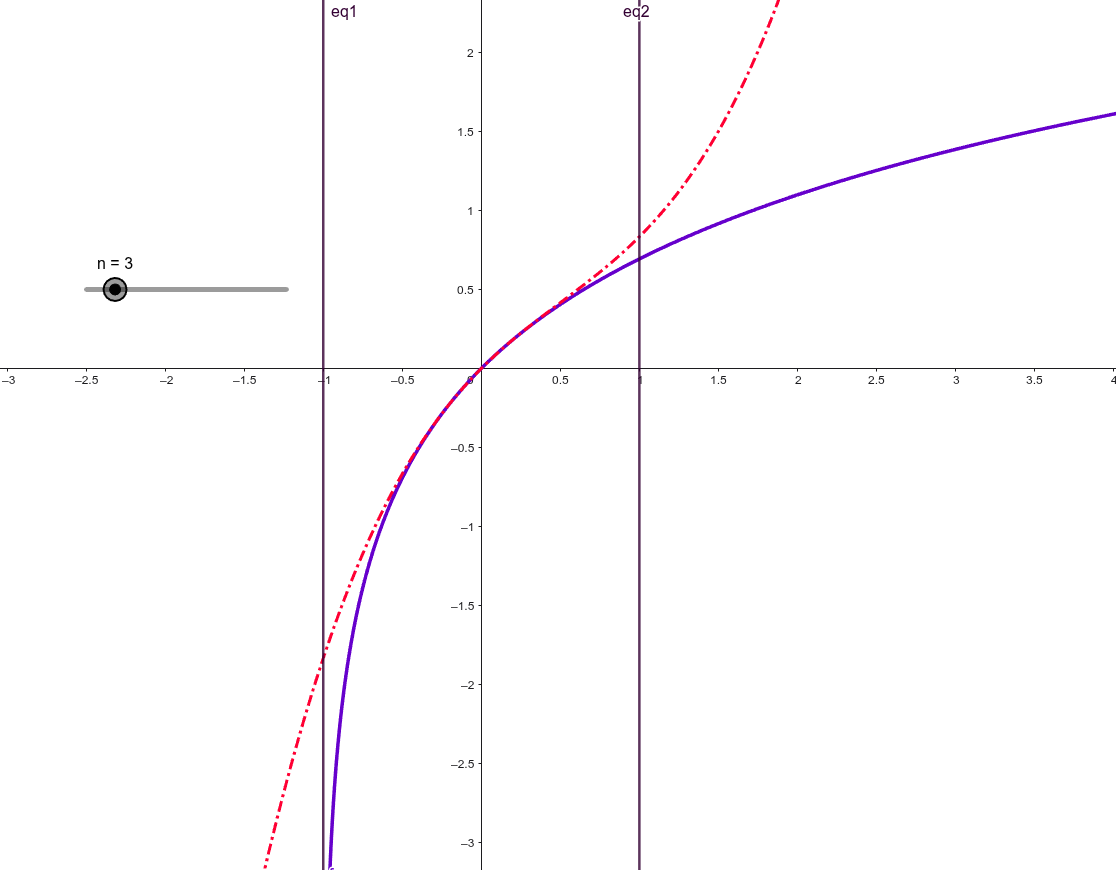
\includegraphics[width=\linewidth]{img/image.png}
    \caption{Comparação da Série de Mercator para $n=3$ e a função $\ln (1+x)$.}
\end{figure}

No GeoGebra, criamos um gráfico animado iterativo para enxergar como a Série de Mercator se aproxima da função $\ln (1+x)$ para $-1< x \le 1$ quando o número de iterações aumenta. Segue o link: 
\href{https://www.geogebra.org/calculator/jyycuaxp}{Clique Aqui}

\section{O Número de Euler e o Logaritmo Natural}

No início do século XVIII, a conexão entre logaritmos e exponenciais foi finalmente reconhecida e o conceito de uma base para um logaritmo foi compreendido.

Em 1748, 101 anos após os trabalhos de Saint Vincent e de Sarasa, Leonhard Euler (1707 - 1753) calculou a base deste logaritmo natural (denominado desta maneira por Mercator). Essa base era nada mais que o número $e$ (número de Euler). A história do número de Euler é um pouco longa, faremos um breve resumo para explicar qual a sua relação com o logarítmo natural.

Em 1683, Jakob Bernoulli (1654-1705), estava estudando sobre a capitalização em juros compostos. Ele observou que ao aumentar a frequência da capitalização (diária, por hora, por minuto, etc.), o montante final aumentava, porém não tendia ao infinito, era limitado. Ele precisou estudar o seguinte limite:

\[
\lim_{n \to \infty}\left(1+\frac{1}{n}\right)^n
\]

O qual conseguiu determinar que estava entre $2$ e $3$, utilizando o teorema do binônimo de Newton.

Algumas décadas depois, em meio do século XVIII, Euler chamou este número de $e$, e conseguiu mostrar, também utilizando o teorema do binômio que

\[
e = \lim_{n \to \infty}\left(1+\frac{1}{n}\right)^n = \sum_{k=0}^{\infty}\frac{1}{k!}
\]

Mas dentro de nosso contexto, o mais interessante que Euler fez, foi mostrar que esse número seria a base do logarítmo hiperbólico (ou natural). Dessa vez, definiremos a área abaixo da hipérbole de $1$ até $a$ como sendo $A(a) = \log_{b} a$, pois agora é compreendida o conceito de base para logaritmo.

Observe que qualquer que seja a base $b$ do logaritmo hipérbolico, ele é tal que $A(b) = \log_{b} b = 1$. Faremos uma construção similar, porém diferente da proposta de Saint-Vincent.

Aproximaremos a área em $n$ retângulos, definindo $q = \sqrt[n]{b}$, então o $k$-ésimo retângulo é tal que o comprimento de sua base vale $q^{k+1} - q^k$ e sua altura é $\dfrac{1}{q^k}$, e portanto, a área de cada retângulo vale
\[
    A_k = \frac{q^{k+1}-q^k}{q^k} = q - 1
\]

\begin{figure}[H]
    \centering
    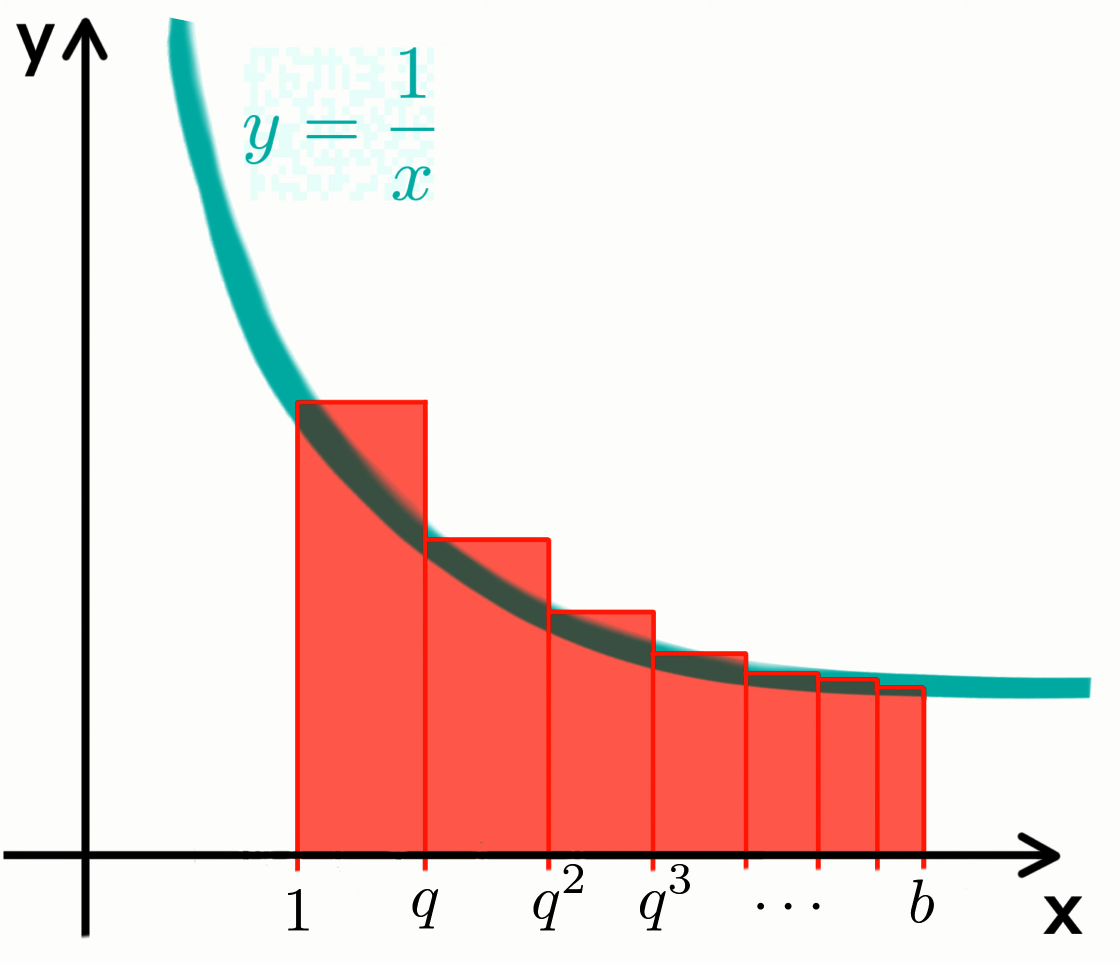
\includegraphics[width=0.5\linewidth]{img/eulerNatural.png}
    \caption{Área da Hipérbole}
    \label{fig:hiperboleeuler}
\end{figure}

Portanto, cada retângulo tem a mesma área $q - 1$, logo, a área total aproximada abaixo da hipérbole é nada mais que $A = n(q-1)$, mas sabemos que quando $n$ cresce, esse número deve tender a $1$, ou seja, $b$ deve ser tal que:

\[
    \lim_{n \to \infty} n(q - 1) = 1 \quad \text{, isto é,} \quad \lim_{n \to \infty} n(\sqrt[n]{b} - 1) = 1
\]

Esta foi a expressão que Euler obteve. É possível mostrar rigorosamente que $b$ deve ser o número $e$. Não o faremos aqui, mas daremos uma razão intuitiva:

Sabemos que deve valer o limite: $\lim_{n \to \infty} n(\sqrt[n]{b} - 1) = 1$. Então, para $n$ grande, temos que:

\[
n \left( \sqrt[n]{b} - 1 \right) \approx 1
\]

\[
\Rightarrow \sqrt[n]{b} - 1 \approx \frac{1}{n} 
\Rightarrow \sqrt[n]{b} \approx 1 + \frac{1}{n}
\]

\[
\Rightarrow b \approx \left( 1 + \frac{1}{n} \right)^n 
\xrightarrow[n \to \infty]{} e
\]

E daí, foi descoberto que $e$ era exatamente a base do logaritmo hiperbólico.
\subsection*{Logaritmo na Atualidade}

O advento do logaritmo natural, consolidado por Leonhard Euler, representou uma mudança de paradigma fundamental na matemática, suplantando a relevância dos sistemas anteriores, como os de John Napier e os logaritmos decimais (base 10). Originalmente, o logaritmo surgiu como uma ferramenta computacional, cujo propósito era simplificar cálculos complexos de multiplicação, divisão e potenciação em uma era pré-computadores. Com o surgimento das calculadoras e computadores, essa função original tornou-se obsoleta. A capacidade de realizar cálculos aritméticos de forma instantânea deslocou o foco do logaritmo: de uma ferramenta de cálculo para um conceito central no desenvolvimento teórico e prático da matemática.

Atualmente, o logaritmo natural está intrinsecamente ligado ao cálculo diferencial e integral. A base $e$ (o número de Euler) possui propriedades matemáticas vantajosas que simplificam enormemente as operações de diferenciação e integração. Como a função $\ln(x)$ é a primitiva de $\frac{1}{x}$ e a inversa da função exponencial $e^x$ (cuja derivada é ela mesma), ela se torna a linguagem natural para descrever e resolver problemas em inúmeras áreas da ciência e engenharia. Assim, o logaritmo deixou de ser uma ferramenta para fazer contas mecânicas e se tornou um pilar para resolver problemas impraticáveis.

A seguir, ilustramos essa mudança de paradigma com uma aplicação fundamental em Inferência Estatística.

\subsubsection*{Exemplo: O Estimador de Máxima Verossimilhança (EMV) da Normal}
Seja $X_1, X_2, \ldots, X_n$ uma amostra aleatória i.i.d. de uma distribuição Normal $N(\mu, \sigma^2)$. A Função de Densidade de Probabilidade (FDP) de cada observação $x_i$ é:
\[
f(x_i \mid \mu, \sigma^2) = \frac{1}{\sqrt{2\pi\sigma^2}} \exp\left( -\frac{(x_i-\mu)^2}{2\sigma^2} \right)
\]

\paragraph{Função de Verossimilhança .}
A função de verossimilhança $L(\mu, \sigma^2 \mid \mathbf{x})$ é o produto das FDPs:
\begin{equation} \label{eq:likelihood}
    L(\mu, \sigma^2 \mid \mathbf{x}) = \left( \frac{1}{2\pi\sigma^2} \right)^{n/2} \exp\left( -\frac{1}{2\sigma^2} \sum_{i=1}^{n} (x_i-\mu)^2 \right)
\end{equation}

\paragraph{Função de Log-Verossimilhança.}
Para encontrar os parâmetros que maximizam a função de verossimilhança, o caminho direto seria derivar a Equação (\ref{eq:likelihood}) em relação a $\mu$ e $\sigma^2$. No entanto, derivar um produto de $n$ funções exponenciais precisaria de aplicações sucessivas e complexas da Regra do Produto, tornando o problema analiticamente complexo.

Daí, o logaritmo demonstra sua usabilidade moderna. A chave para sua aplicação é que por ser uma função estritamente crescente, encontrar os pontos críticos de $L(\theta)$ é equivalente a encontrar os pontos críticos de $\ln(L(\theta))$. Ao aplicar o logaritmo natural, transformamos o produto complexo em uma soma factível, a log-verossimilhança $\ell(\mu, \sigma^2)$:
\begin{align*}
    \ell(\mu, \sigma^2 \mid \mathbf{x}) &= \ln\left[ L(\mu, \sigma^2 \mid \mathbf{x}) \right] \\
    &= -\frac{n}{2} \ln(2\pi) - \frac{n}{2} \ln(\sigma^2) - \frac{1}{2\sigma^2} \sum_{i=1}^{n} (x_i-\mu)^2
\end{align*}

\paragraph{Maximização.}
Agora, derivar esta soma em relação a $\mu$ e $\sigma^2$ e igualar a zero torna-se uma tarefa simples de cálculo. Resolvendo o sistema de equações resultante, encontramos os EMVs:
\begin{itemize}
    \item \textbf{Para a média $\mu$:} A média amostral.
          \[ \hat{\mu}_{ML} = \bar{x} = \frac{1}{n}\sum_{i=1}^{n} x_i \]
    \item \textbf{Para a variância $\sigma^2$:} A variância amostral com denominador $n$.
          \[ \hat{\sigma}^2_{ML} = \frac{1}{n}\sum_{i=1}^{n} (x_i-\bar{x})^2 \]
\end{itemize}

Portanto, o exemplo demonstra perfeitamente a "nova" aplicação do logaritmo. Ele não foi usado para facilitar um cálculo aritmético, mas sim para transformar um problema analítico hercúlico em um que é solucionável. O logaritmo deixou de ser uma ferramenta para o cálculo mecânico para se tornar uma ferramenta indispensável para a simplificação da própria análise matemática.
\subsection{Escala Richter: Da Amplitude à Escala Destrutiva}
Durante os noticiários sobre desastres naturais, frequentemente a intensidade dos terremotos é quantificada por um número na Escala de Magnitude Richter com o intuito de evidenciar a magnitude da perda material e humanitária encadeada pela energia liberada do tremor.

Mas afinal, como surgiu e como interpreto a escala? Desenvolvida em meados da década de 1930 pelos pesquisadores Charles Richter e Beno Gutenberg, da Caltech, a Escala Richter originou-se da necessidade de condensar um conjunto denso de dados de um sismógrafo em um único número, de forma concisa e intuitiva. Para isso, propuseram a seguinte fórmula:

\begin{equation}
    M = \log_{10}\left(\frac{A}{A_0}\right)
\end{equation}

onde $A$ é a amplitude máxima da onda sísmica registrada e $A_0$ é uma amplitude de referência. É importante notar que $A_0$ não é uma constante; seu valor depende da distância entre o sismógrafo e o epicentro do terremoto.

Em virtude da natureza logarítmica da fórmula, um acréscimo de apenas uma unidade na escala não representa um aumento linear, mas sim um aumento exponencial na intensidade do tremor. Aplicando a definição de logaritmo, podemos isolar a amplitude $A$:

\begin{equation}
    M = \log_{10}\left(\frac{A}{A_0}\right) \iff A = 10^{M} \cdot A_0
\end{equation}

Para compreender melhor, podemos comparar a amplitude de um terremoto de magnitude $M$ (denotaremos a amplitude do tremor com magnitude $M$ por meio de $A_M$) com a de um terremoto de magnitude $M+1$:

\begin{equation*}
\begin{cases}
    A_M = 10^{M} \cdot A_0 \\
    A_{M+1} = 10^{M+1} \cdot A_0
\end{cases}
\quad\Longrightarrow\quad A_{M+1} = 10 \cdot A_M
\end{equation*}

Daí, vemos que o aumento de apenas um ponto na Escala Richter corresponde a um tremor com amplitude 10 vezes maior.

Ademais, perceba que tal resultado é referente ao tremor e não necessariamente sobre sua capacidade destrutiva. Dessa maneira, a fim de ilustrar o potencial destrutivo do acréscimo de uma unidade na Escala Richter introduziremos o conceito de energia:

\begin{equation*}
    E_M \propto A^{3/2} \iff E_M = k \cdot A^{3/2}
\end{equation*}

Denotando a energia liberada por um terremoto de escala $M+1$ por $E_{M+1}$, temos que:

\begin{align*}
    E_{M+1} &\propto (A_{M+1})^{3/2} \\
            &= (10 \cdot A_M)^{3/2} \\
            &= 10^{3/2} \cdot (A_M)^{3/2} \\
            &\propto 10^{3/2} \cdot E_M
\end{align*}

Perceba que, $10^{3/2} \approx 31,6$, isto é, a capacidade destrutiva do tremor é 31,6 vezes maior ao aumentar uma unidade na escala, e o impacto sobre a realidade pode ser percebido através da seguinte tabela:

\begin{table}[H]
\centering
\label{tab:richter_simples}
\begin{tabular}{|c|l|}
    \hline
\textbf{Magnitude} & \textbf{Descrição dos Efeitos} \\
\hline
1--3 & Nada / Imperceptível \\
3--4 & Perceptível, sem danos \\
4--5 & Danos domésticos \\
5--6 & Danos em prédios sem estrutura adequada \\
6--7 & Danos em prédios normais \\
7--8 & Danos sérios \\
8--9 & Destruição de cidades \\
9--10 & Muda a topografia \\
$>10$ & Desconhecido / Catástrofe global \\
\hline
\end{tabular}
\caption{Efeitos por Magnitude na Escala Richter}
\end{table}



Fica claro, portanto, que o conceito introduzido por John Napier em 1614 transcende a matemática abstrata. O real conhecimento dos logaritmos permite uma análise crítica da realidade. Diferentemente do que o senso comum poderia sugerir, um terremoto de magnitude 10 não causa o dobro da destruição de um de magnitude 5. Na verdade, seu poder destrutivo é cerca de 31 milhões de vezes maior. Ter essa percepção nos ajuda a compreender melhor a magnitude dos fenômenos que nos rodeiam e analisá-los com senso crítico.

\subsection{Potencial Hidrogeniônico (pH)}

A escala de pH (Potencial Hidrogeniônico) é um conceito bastante estudado em química. Esse conceito foi definido pelo químico dinamarquês Soren Peter Lauritz Sorensen no ano de 1909. Ela serve para determinar os níveis de acidez de uma solução. O pH de uma solução é definido como o logaritmo decimal do inverso da concentração de $H_3O^{+}$ (ion hidroxônio), ou seja,

\[
pH = - \log[H_3O^{+}]
\]

Assim, percebe-se que quanto maior o valor da concentração de $H_3O^{+}$, menor o valor do pH, ou seja, quanto mais ácida a solução, menor o pH. Definir a acidez em uma escala logarítimica foi muito positivo. Primeiro que, em solução, os valores de íons hidrogênio podem variar drasticamente, além de serem, na maioria das vezes, expressos em potências negativas de 10.


A classificação do pH se dá da seguinte forma:

\begin{center}
\begin{tabular}{|c|c|}
\hline
\textbf{pH} & \textbf{solução} \\
\hline
0 a 7 & ácida \\
\hline
7 & neutra \\
\hline
7 a 14 & básica \\
\hline
\end{tabular}
\end{center}

% \begin{figure}[H]
%     \centering
%     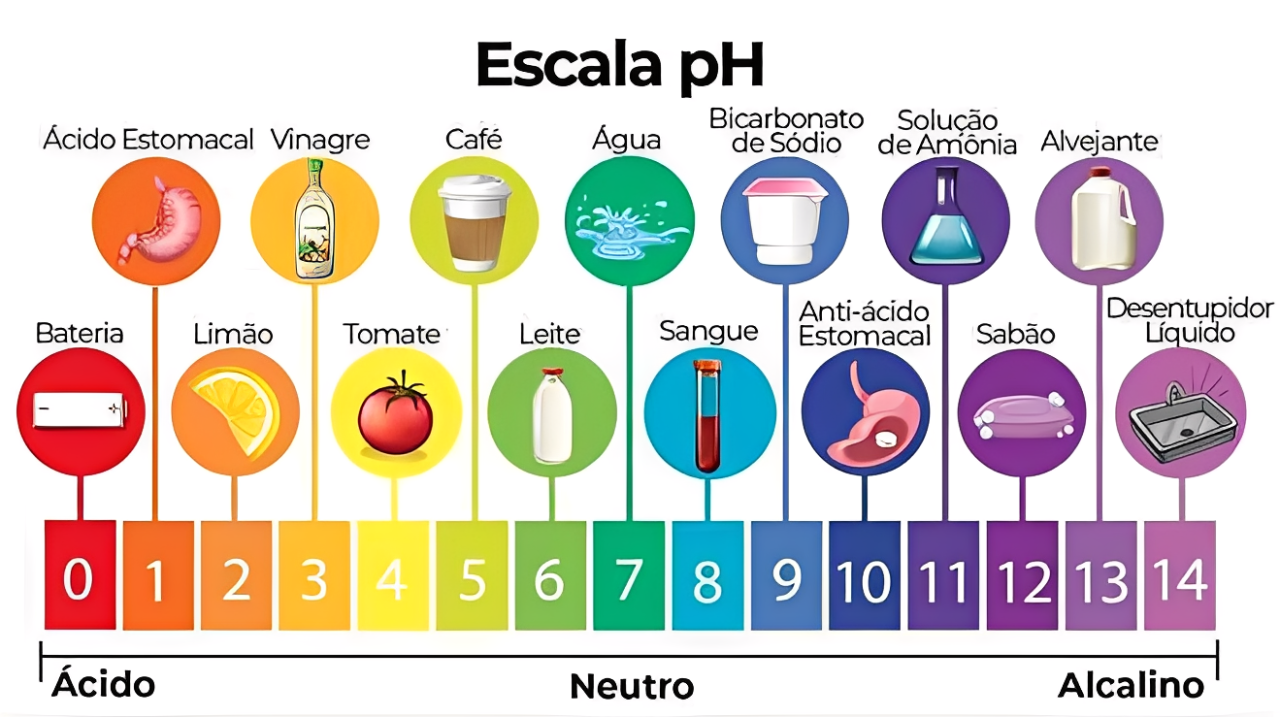
\includegraphics[width=\linewidth]{img/escalaph.jpg}
%     \caption{Escala pH}
% \end{figure}
Abaixo temos uma imagem com o pH de algumas soluções mais comuns.

\begin{figure}[h]
    \centering
    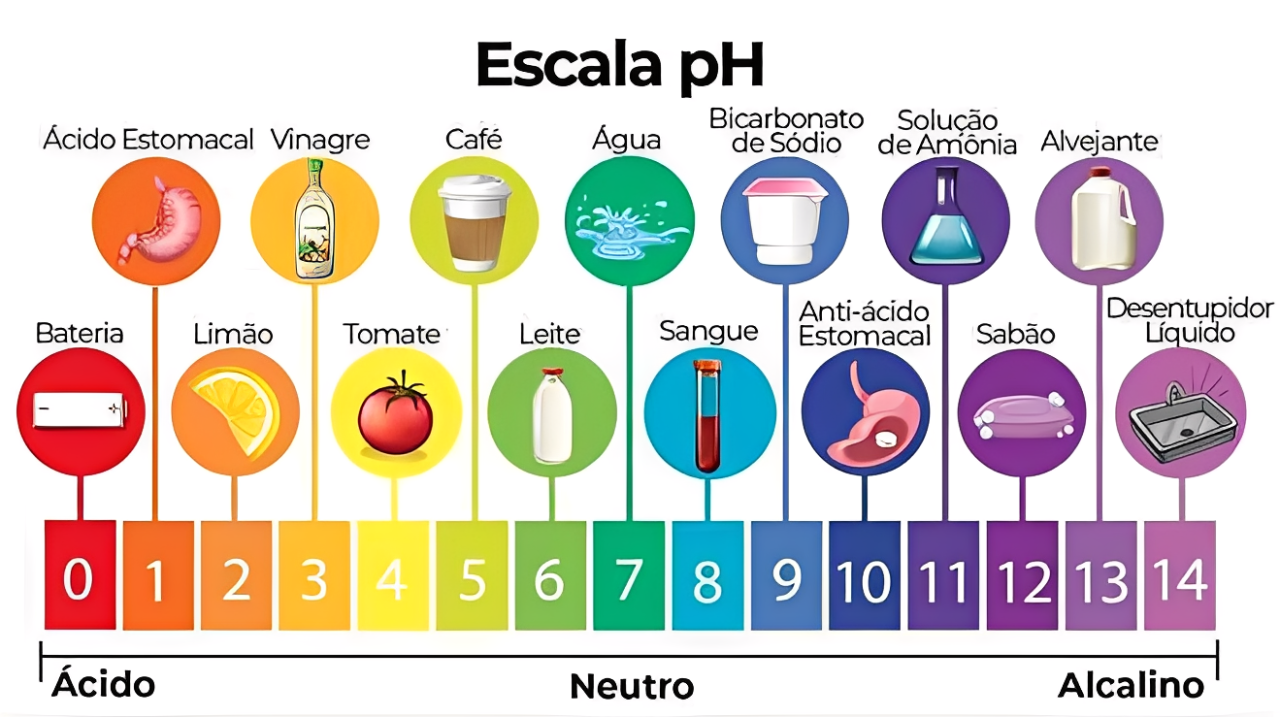
\includegraphics[width=0.9\textwidth]{img/escalaph.png}
    \caption{Exemplos de soluções e seu pH}
    \label{fig:escalaph}
\end{figure}


\textbf{Exemplo.} Jean, um químico curioso, estava na praia e enche um copo com água do mar. Ao chegar em seu laboratório, ele mede a concentração de íons ($H_3O^{+}$) desse copo de água, obteve-se que esta é de $10^{-8}$ mol/l. Assim qual será o pH dessa água? 

\begin{align*}
pH &= -\log[H_3O^+], \\
pH &= -\log 10^{-8}, \\
pH &= -(-8) \log 10, \\
pH &= 8
\end{align*}

Assim, Jean notou que a água do mar era uma solução básica.



\section{Questão Proposta}

Seja $f:\mathbb{R}_{>0} \to \mathbb{R}$ função contínua tal que $f(xy) = f(x) + f(y)$, o objetivo desta questão é mostrar que $f(x) = f(e)\text{ln}(x)$.
\begin{enumerate}[(a)]
    \item Mostre que $f(e^n) = n\cdot f(e) \, \forall n \in \mathbb{N}$
    \item Mostre que $f(e^q) = q\cdot f(e) \, \forall q \in \mathbb{Q}_{>0}$
    \item Conclua por continuidade que vale $f(e^r) = r\cdot f(e) \, \forall r \in \mathbb{R}_{>0}$ e portanto deve-se ter $f(x) = f(e) \text{ln}(x)$.
\end{enumerate}

Dica: Para o item (c) você deve utilizar dois resultados importantes vistos em um curso de análise real:
\begin{enumerate}
    \item $f$ é contínua em $a$ se para toda sequência $x_n$ convergente a $a$, tem-se $\lim f(x_n) = f(a)$
    \item Os racionais são densos na reta, isto é, para todo número real $r$, existe uma sequência $q_n$ de racionais convergente a $r$
\end{enumerate}





\end{document}